\chapter{Building Block View (Static View)}

\section{Overview}

\begin{center}
	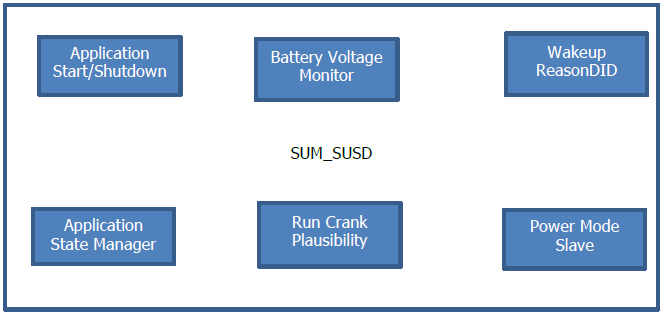
\includegraphics[width=\textwidth]{images/susd_overview}
\end{center}

\subsection{Application State Manager}
\begin{itemize}
\item Coordinate the ECUs operational state with BswM (which controls EcuM)
\item Monitor the Power Moding Slave
\item Perform the logic to determine when to request a change to the ECU's operational state to BswM (from Run to Sleep, Reset, or Off)
\item Request BswM to shut down (to the shutdown target) when all SW-Cs have enabled shutdown
\item Request BswM to remain in "run" when at least one SW-C has not enabled shutdown
\item Notify SUM_SOH of any shutdown attempts
\end{itemize}

\subsection{Application Start/Shutdown}
\begin{itemize}
\item Maintain list of active ECU initiated system wakeups
\item Map of SW-Cs to ECU wakeups
\item Poll of EcuM for wakeup request on behalf of SW-C
\item Coordinate of all SW-C startup notifications
\item Coordinate of all SW-C shutdown notifications
\item Disable / Enable future Wakeups based on the ECU's needs (based on vehicle modes or functional needs)
\item Handle faults for wakeups, and disable future wakeup source for subsequent cycles
\item Provide Notification to other SW-C to Disable DTCs for \code{DisableDTCBatteryWakeupPeriod} following wakeup from Battery event
\end{itemize}

\subsection{Battery Voltage Monitor}
\begin{itemize}
\item Process Battery Voltage Input
\item Monitor Battery Voltage State of Charge serial data signal - TBD
\item Provide Notification to SW-C of standardized voltage ranges: Normal, Overvoltage, Undervoltage
\item Provide an actual battery voltage value
\item Provide Notification to other SW-C to Disable DTCs based on Battery Voltage
\end{itemize}

\subsection{Power Mode Slave}
\begin{itemize}
\item Process Signals from Power Mode Master and Backup Power Mode Master
\item Handle Error notification for fault handling of Power Mode Signal Usage
\item Provide PropulsionStatus Notification
\item Calculate ECU specific power moding state based on internal and external inputs
\item Provide Vehicle Power Mode Notification for Application, DIDs etc
\end{itemize}

\subsection{Run/Crank Plausibility}
\begin{itemize}
\item Monitor Run Crank input from local I/O
\item Perform RunCrank Status Calculation based on I/O and Power Moding Inputs
\item Handle faults with Run / Crank detection
\end{itemize}

\subsection{BSW Module Interaction}
\begin{itemize}
\item BswM, Dem, Dcm and Com are used by SUSD for its functionality. 
\item BswM is used to monitor ECU states and request ECU states, accept reset request, disable wakeup and get DTC information. 
\item Dem is used for Vehicle power mode, SetEvent Status
\item Dcm for DIDs
\item NvM is used to store persistent data across ECU power cycles.
\end{itemize}

\Requirement{250}
{
SUM\_SUSD is who instances the RAM mirror blocks for NvM (E0D7 Activity Records block, FirstBootPostFlash block, E0D7 MonitorDisabled block, ECU Wakeup Detection Records block, and RESETExecution Timer block). SUM\_SUSD shall ensure that the pointer passed to any RTE NvM API call (WriteBlock, SetRamBlockStatus) is never a null pointer, so that no null pointer exception is caused for this scenario.
SUM\_SUSD satisfies this by declaring all NvM RAM block variables as statically allocated objects (compile-time guarantee), and by passing their addresses directly to the NvM access struct initializers.
}
{\Satisfies{SRS_SUSD 334} \Satisfies{rta_sum_ffi 001}}

\section{Configuration}

SUM_SUSD is a SWC within the context of AUTOSAR.
It consists of static files and generated files.
SUM_SUSD configuration is done the same way as for standard BSW modules.
A parameter definition file is included with the module which allows users to configure the available parameters.
The generated files change based on the configuration.

\begin{itemize}
\item The configuration parameters for SUSD are provided in \file{SUM_SUSD_EcucParamdef.arxml}.
The user shall configure the various parameters provided in the paramdef.
Based on the inputs configured, SUSD shall use OAW scripts to generate the source and header files along with the Software Component Description ARXML.
\item Based on the configuration of parameters in container \code{SUSDSUMInterfaces}, SUM ports and interfaces for Permit Execution and Shutdown Permission shall be created in SWCD arxml.
\item Based on the configuration of parameters in container \code{SUSD_SWCInfo}, SWC interfaces and ports for various functionalities shall be created in SWCD.
\item The string parameters are provided for the names of API and SWCs.
\end{itemize}

\subsection{Included Containers:}

\input{generated/tables/containers.tex}

\subsection{SUSDGeneral}
\label{subsection:SUSDGen}

\Requirement{003}
{\ConfigurationParameter{SUSD_t_Shutdown_Refresh}
{Time in sec, for which a SW-C with a ShutdownPermission interface, shall refresh its signal for that interface.}
{1..1}
{ECUC-FLOAT-PARAM-DEF}
{0.001..0.5}
{0.1}}
{\Satisfies{SRS_SUSD 019} \Satisfies{SRS_SUSD 018} \Satisfies{SRS_SUSD 115}}

\Requirement{004}
{\ConfigurationParameter{SUSD_t_Force_Shutdown_Wait}
{Time in sec for which SUSD shall wait before requesting Shutdown from BswM, after indicating to all SW-Cs with PermitExecution interface to Shutdown.}
{1..1}
{ECUC-FLOAT-PARAM-DEF}
{0..65.535}
{0}}
{\Satisfies{SRS_SUSD 115}}

\Requirement{139}
{\ConfigurationParameter{SUSD_t_Battery_Periodicity}
{Time in msec, for the periodicity of notifying SW-C of changes to the Battery Monitors.}
{1..1}
{ECUC-INTEGER-PARAM-DEF}
{1..500}
{100}}
{\Satisfies{SRS_SUSD 115}}

\ConfigurationParameter{SUSD_t_VehiclePowerMode_Periodicity}
{Time in msec, for the periodicity of notifying SW-C of changes to the Vehicle Power Mode.}
{1..1}
{ECUC-INTEGER-PARAM-DEF}
{1..500}
{100}

{\ConfigurationParameter{SUSD_t_RunCrank_Periodicity}
{Time in msec, for the periodicity of notifying SW-C of changes to the Run Crank.}
{1..1}
{ECUC-INTEGER-PARAM-DEF}
{1..500}
{100}

\Requirement{140}
{\ConfigurationParameter{SUSD_t_Wakeup_Periodicity}
{Time in msec, for the periodicity of Wake up polling.}
{1..1}
{ECUC-INTEGER-PARAM-DEF}
{1..500}
{100}}
{\Satisfies{SRS_SUSD 115}}

\Requirement{141}
{\ConfigurationParameter{SUSD_t_AppManager_Periodicity}
{Time in msec, for the periodicity of AppStateManager.}
{1..1}
{ECUC-INTEGER-PARAM-DEF}
{1..500}
{100}}
{\Satisfies{SRS_SUSD 115}}

\ConfigurationParameter{SUSD_PowerModing_Slave_Supported}
{Whether the ECU is a Power Moding Slave.}
{1..1}
{ECUC-BOOLEAN-PARAM-DEF}
{TRUE, FALSE}
{FALSE}}

\ConfigurationParameter{SUSD_RunCrankPlausibility_Supported}
{Whether the RunCrank Input is available from one of the software components.}
{1..1}
{ECUC-BOOLEAN-PARAM-DEF}
{TRUE, FALSE}
{FALSE}

\Requirement{005}
{\ConfigurationParameter{SUSD_C_DefaultShutdownState}
{The default ECU operation state when shutting down.}
{1..1}
{ECUC-ENUMERATION-PARAM-DEF}
{Off, Sleep}
{}}
{\Satisfies{SRS_SUSD 021} \Satisfies{SRS_SUSD 115}}


\ConfigurationParameter{SUM_SUSD_RESETExecution_TIMER_Thresh_Init}
{Initial value of the Calibration parameter SUM_SUSD _RESETExecution_TIMER_Thresh.}
{1..1}
{ECUC-INTEGER-PARAM-DEF}
{0..10}
{10}

\ConfigurationParameter{SUSD_VPM_ASIL_A_Supported}
{This parameter shall control the determination of Vehicle Power Mode at ASIL A or QM level.
If set to False, then VPM shall be calculated without Failed Safety signals.}
{1..1}
{ECUC-BOOLEAN-PARAM-DEF}
{TRUE, FALSE}
{FALSE}

\ConfigurationParameter{SUSD_VPM_Cybersecurity_Supported}
{This parameter shall control the determination of Vehicle Power Mode with or without Cybersecurity.
If set to False, then VPM shall be calculated without Failed Security signals.}
{1..1}
{ECUC-BOOLEAN-PARAM-DEF}
{TRUE, FALSE}
{FALSE}

\ConfigurationParameter{SUSD_VPM_SPM_Initial}
{Initial value for System Power Mode used for Vehicle Power Mode determination when a valid System Power Mode has not been received yet.}
{1..1}
{ECUC-ENUMERATION-PARAM-DEF}
{SUM_PMS_OFF, SUM_PMS_ACCESSORY, SUM_PMS_RUN, SUM_PMS_STARTREQUEST, SUM_PMS_PROPULSION, SUM_PMS_TRANSPORT}
{SUM_PMS_OFF}

\ConfigurationParameter{SUSD_VPM_SBPM_Initial}
{Initial value for System Backup Power Mode used for Vehicle Power Mode determination when a valid System Backup Power Mode has not been received yet.}
{1..1}
{ECUC-ENUMERATION-PARAM-DEF}
{SUM_PMS_OFF, SUM_PMS_ACCESSORY, SUM_PMS_RUN, SUM_PMS_STARTREQUEST, SUM_PMS_PROPULSION, SUM_PMS_TRANSPORT}
{SUM_PMS_OFF}

\ConfigurationParameter{SUSD_PermitExecAvailable}
{A parameter for Permit Execution Interface for this SWC.}
{1..1}
{ECUC-BOOLEAN-PARAM-DEF}
{TRUE, FALSE}
{TRUE}

\Requirement{015}
{\ConfigurationParameter{SUSD_DisNvMWriteAvailable}
{A parameter for Disable NvM Write Interface for this SWC}
{0..1}
{ECUC-BOOLEAN-PARAM-DEF}
{TRUE, FALSE}
{TRUE}}
{\Satisfies{SRS_SUSD 039}}

\ConfigurationParameter{SUSD_ECUOpStateDIDSupported}
{This parameter created to provide user the option to choose ECU Operating State DID as optional.}
{1..1}
{ECUC-BOOLEAN-PARAM-DEF}
{TRUE, FALSE}
{TRUE}

\ConfigurationParameter{SUSD_Battery_State_of_Charge_Supported}
{This parameter must be set equal to true if the ECU has an input which monitors the vehicle battery state of charge.}
{1..1}
{ECUC-BOOLEAN-PARAM-DEF}
{TRUE, FALSE}
{FALSE}

\ConfigurationParameter{SUSD_BatteryVoltageDIDSigRef}
{Reference to DID for Battery Voltage Signal.}
{1..1}
{ECUC-REFERENCE-DEF}
{Project specific}
{}

\Requirement{158}
{\ConfigurationParameter{SusdEcuWakeUpDetectionRecordsNvmBlockRef}
{Reference to NVM Block for storing ECU Wakeup Detection Records.}
{1..1}
{ECUC-REFERENCE-DEF}
{N/A}
{}}
{\Satisfies{SRS_SUSD 271}}

\ConfigurationParameter{SUSD_WakeupSourceReasonDIDSigRef}
{Reference to DID for Wakeup Source Reason Signal.}
{0..1}
{ECUC-CHOICE-REFERENCE-DEF}
{Project specific}
{}

\ConfigurationParameter{SUSD_ActiveWakeupSourceDIDSigRef}
{Reference to DID for Active Wakeup Source(s) Signal.}
{0..1}
{ECUC-CHOICE-REFERENCE-DEF}
{Project specific}
{}


\ConfigurationParameter{SUSD_ECUOperatingStateDIDSigRef}
{Reference to DID for ECU Operating State Signal.}
{0..1}
{ECUC-CHOICE-REFERENCE-DEF}
{Project specific}
{}

\ConfigurationParameter{SUSD_PowerModingStateDIDSigRef}
{Reference to DID for Power Moding State Signal.}
{0..1}
{ECUC-CHOICE-REFERENCE-DEF}
{Project specific}
{}

\ConfigurationParameter{SUSD_VehiclePowerModeInvalidityDIDSigRef}
{Reference to DID for Vehicle Power Mode Invalidity Signal.}
{0..1}
{ECUC-CHOICE-REFERENCE-DEF}
{Project specific}
{}

\ConfigurationParameter{SUSD_DemDataElementClass_VPwrSetEnCondDataSigRef}
{Reference to Dem Data Element Class for Vehicle Power Set Enable Condition Data Signal.}
{0..1}
{ECUC-CHOICE-REFERENCE-DEF}
{Project specific}
{}

\ConfigurationParameter{SUM_SUSD_RESETExecution_TIMERNvmBlockRef}
{Reference to NVM Block for storing SUM_SUSD_RESETExecution_TIMER.}
{1..1}
{ECUC-CHOICE-REFERENCE-DEF}
{Project specific}
{}

\ConfigurationParameter{Sum_SUSD_Sig_PrimaryPowerMode_Ref}
{Reference to com Signal for Primary Power Mode.}
{1..1}
{ECUC-FOREIGN-REFERENCE-DEF}
{Project specific}
{}

\ConfigurationParameter{Sum_SUSD_Sig_BackupPowerMode_Ref}
{Reference to com Signal for Backup Power Mode.}
{1..1}
{ECUC-FOREIGN-REFERENCE-DEF}
{Project specific}
{}

\ConfigurationParameter{Sum_SUSD_ServiceBased_PMM_Ref}
{Reference to service-based PMM interface.}
{0..1}
{ECUC-FOREIGN-REFERENCE-DEF}
{Project specific}
{}

\ConfigurationParameter{Sum_SUSD_ServiceBased_BPMM_Ref}
{Reference to service-based BPMM interface.}
{0..1}
{ECUC-FOREIGN-REFERENCE-DEF}
{Project specific}
{}

\ConfigurationParameter{Sum_SUSD_ServiceBased_DatatypeMappingSet}
{Reference to service-based datatype mapping set for service based PMM and BPMM.}
{0..1}
{ECUC-CHOICE-REFERENCE-DEF}
{Project specific}
{}

\subsection{SUSDWakeUpRelation}
\label{subsection:SUSDWake}

\Requirement{007}
{\ConfigurationParameter{SUSD_WakeupSourceId}
{This parameter defines the identifier of this wakeup source.}
{1..*}
{ECUC-REFERENCE-DEF}
{}
{}}
{\Satisfies{SRS_SUSD 051} \Satisfies{SRS_SUSD 057} \Satisfies{SRS_SUSD 058}}

\subsection{SUSDSUMInterfaces}

\Requirement{008}
{\ConfigurationParameter{SUSD_PNCPermExec}
{Enables or disables the Permit Execution interface to PNC.}
{1..1}
{ECUC-BOOLEAN-PARAM-DEF}
{TRUE, FALSE}
{TRUE}}
{\Satisfies{SRS_SUSD 040} \Satisfies{SRS_SUSD 041}}

\Requirement{009}
{\ConfigurationParameter{SUSD_LNMPermExec}
{Enables or disables the Permit Execution interface to LNM.}
{1..1}
{ECUC-BOOLEAN-PARAM-DEF}
{TRUE, FALSE}
{TRUE}}
{\Satisfies{SRS_SUSD 049} \Satisfies{SRS_SUSD 050}}

\Requirement{010}
{\ConfigurationParameter{SUSD_ERRHPermExec}
{Enables or disables the Permit Execution interface to ERRH.}
{1..1}
{ECUC-BOOLEAN-PARAM-DEF}
{TRUE, FALSE}
{TRUE}}
{\Satisfies{SRS_SUSD 042} \Satisfies{SRS_SUSD 043}}

\Requirement{011}
{\ConfigurationParameter{SUSD_SOHPermExec}
{Enables or disables the Permit Execution interface to SOH.}
{1..1}
{ECUC-BOOLEAN-PARAM-DEF}
{TRUE, FALSE}
{TRUE}}
{\Satisfies{SRS_SUSD 047} \Satisfies{SRS_SUSD 048}}

\Requirement{012}
{\ConfigurationParameter{SUSD_TCSPermExec}
{Enables or disables the Permit Execution interface to TCS.}
{1..1}
{ECUC-BOOLEAN-PARAM-DEF}
{TRUE, FALSE}
{TRUE}}
{\Satisfies{SRS_SUSD 044}}

\Requirement{013}
{\ConfigurationParameter{SUSD_SSCPermExec}
{Enables or disables the Permit Execution interface to SSC.}
{1..1}
{ECUC-BOOLEAN-PARAM-DEF}
{TRUE, FALSE}
{TRUE}}
{\Satisfies{SRS_SUSD 045}}

\Requirement{014}
{\ConfigurationParameter{SUSD_SSMPermExec}
{Enables or disables the Permit Execution interface to SSM.}
{1..1}
{ECUC-BOOLEAN-PARAM-DEF}
{TRUE, FALSE}
{TRUE}}
{\Satisfies{SRS_SUSD 046}}

\ConfigurationParameter{SUSD_SrvcMgrPermExec}
{Enables or disables the Permit Execution interface to SrvcMgr.}
{1..1}
{ECUC-BOOLEAN-PARAM-DEF}
{TRUE, FALSE}
{TRUE}

\ConfigurationParameter{SUSD_DIAGPermExec}
{Enables or disables the Permit Execution interface to DIAG.}
{1..1}
{ECUC-BOOLEAN-PARAM-DEF}
{TRUE, FALSE}
{TRUE}

\ConfigurationParameter{SUSD_SPMPermExec}
{Enables or disables the Permit Execution interface to SPM.}
{1..1}
{ECUC-BOOLEAN-PARAM-DEF}
{TRUE, FALSE}
{TRUE}

\ConfigurationParameter{SUSD_PNCShutdownPerm}
{Enables or disables the Shutdown Permission interface to PNC.}
{1..1}
{ECUC-BOOLEAN-PARAM-DEF}
{TRUE, FALSE}
{TRUE}

\ConfigurationParameter{SUSD_LNMShutdownPerm}
{Enables or disables the Shutdown Permission interface to LNM.}
{1..1}
{ECUC-BOOLEAN-PARAM-DEF}
{TRUE, FALSE}
{TRUE}

\ConfigurationParameter{SUSD_ERRHShutdownPerm}
{Enables or disables the Shutdown Permission interface to ERRH.}
{1..1}
{ECUC-BOOLEAN-PARAM-DEF}
{TRUE, FALSE}
{TRUE}

\ConfigurationParameter{SUSD_SOHShutdownPerm}
{Enables or disables the Shutdown Permission interface to SOH.}
{1..1}
{ECUC-BOOLEAN-PARAM-DEF}
{TRUE, FALSE}
{TRUE}

\ConfigurationParameter{SUSD_DIAGShutdownPerm}
{Enables or disables the Shutdown Permission interface to DIAG.}
{1..1}
{ECUC-BOOLEAN-PARAM-DEF}
{TRUE, FALSE}
{TRUE}

\ConfigurationParameter{SUSD_TCSShutdownPerm}
{Enables or disables the Shutdown Permission interface to TCS.}
{1..1}
{ECUC-BOOLEAN-PARAM-DEF}
{TRUE, FALSE}
{TRUE}

\ConfigurationParameter{SUSD_SrvcMgrShutdownPerm}
{Enables or disables the Shutdown Permission interface to SrvcMgr.}
{1..1}
{ECUC-BOOLEAN-PARAM-DEF}
{TRUE, FALSE}
{TRUE}

\ConfigurationParameter{SUSD_SSCShutdownPerm}
{Enables or disables the Shutdown Permission interface to SSC.}
{1..1}
{ECUC-BOOLEAN-PARAM-DEF}
{TRUE, FALSE}
{TRUE}

\ConfigurationParameter{SUSD_SSMShutdownPerm}
{Enables or disables the Shutdown Permission interface to SSM.}
{1..1}
{ECUC-BOOLEAN-PARAM-DEF}
{TRUE, FALSE}
{TRUE}

\ConfigurationParameter{SUSD_SPMShutdownPerm}
{Enables or disables the Shutdown Permission interface to SPM.}
{1..1}
{ECUC-BOOLEAN-PARAM-DEF}
{TRUE, FALSE}
{TRUE}

\subsection{SUSDConfigSet}

\subsubsection{SUSD_C_SWCInfo}

\ConfigurationParameter{SUSD_SWCName}
{String to indicate the SWC name for interface to map the ports in SWC-D}
{0..1}
{ECUC-STRING-PARAM-DEF}
{}
{}

\Requirement{016}
{\ConfigurationParameter{SUSD_C_ShutdownPermControl}
{A boolean calibration parameter for each shutdown permission interface to control the processing of its permissions.}
{1..1}
{ECUC-BOOLEAN-PARAM-DEF}
{TRUE, FALSE}
{TRUE}}
{\Satisfies{SRS_SUSD 024} \Satisfies{SRS_SUSD 116}}

\Requirement{173}
{\ConfigurationParameter{SUSD_BatteryVoltageRangeRef}
{Reference to Battery Voltage Range}
{0..1}
{ECUC-REFERENCE-DEF}
{N/A}
{}}
{\Satisfies{SRS_SUSD 111}}


\subsubsection{SUSDDiagReferences}
\label{sec:Dcmreference}
\Requirement{156}
{\ConfigurationParameter{SusdEcuWakeupDetectionRecordsDidRef}
{Reference to DID 0xF09E "ECU Wakeup Detection Records"}
{1..1}
{ECUC-REFERENCE-DEF}
{N/A}
{}}
{\Satisfies{SRS_SUSD 277}}

\Requirement{157}
{\ConfigurationParameter{SusdRid41ARef}
{Reference to RID 0x41A "Clear ECU Wakeup Detection Records"}
{1..1}
{ECUC-REFERENCE-DEF}
{N/A}
{}}
{\Satisfies{SRS_SUSD 278} \Satisfies{SRS_SUSD 279}}

\Requirement{243}
{\ConfigurationParameter{Did_F089_Reference}
{Did_F089_Reference}
{1..1}
{ECUC-REFERENCE-DEF}
{N/A}
{}}
{\Satisfies{SRS_SUSD 330}}

\subsubsection{SUSD_BatteryVoltageRange}

\Requirement{171}
{\ConfigurationParameter{SUSD_C_DefaultUnderVoltage_hysteresis}
{A float calibration parameter for the hysteresis for the under voltage range in volts and used with default range 9V to 16V.}
{1..1}
{ECUC-FLOAT-PARAM-DEF}
{0..0.5}
{}}
{\Satisfies{SRS_SUSD 028} \Satisfies{SRS_SUSD 116}}

\Requirement{172}
{\ConfigurationParameter{SUSD_C_DefaultOverVoltage_hysteresis}
{A float calibration parameter for the hysteresis for the over voltage range in volts and used with default range 9V to 16V.}
{1..1}
{ECUC-FLOAT-PARAM-DEF}
{0..0.5}
{}}
{\Satisfies{SRS_SUSD 028} \Satisfies{SRS_SUSD 116}}

\paragraph{SUSD_C_BatteryVoltageRange}
This SUSD_C_BatteryVoltageRange container includes parameters related to Battery Voltage Range

\Requirement{174}
{\ConfigurationParameter{SUSD_C_BatteryVoltageRange_Min}
{The minimum voltage in the range}
{1..1}
{ECUC-FLOAT-PARAM-DEF}
{3..28.5}
{9}}
{\Satisfies{SRS_SUSD 111}}

\Requirement{170}
{\ConfigurationParameter{SUSD_C_BatteryVoltageRange_Max}
{The maximum voltage in the range}
{1..1}
{ECUC-FLOAT-PARAM-DEF}
{3..28.5}
{16}}
{\Satisfies{SRS_SUSD 111}}

\Requirement{017}
{\ConfigurationParameter{SUSD_C_UnderVoltage_hysteresis}
{A float calibration parameter for the hysteresis for the under voltage range in volts.}
{1..1}
{ECUC-FLOAT-PARAM-DEF}
{0..0.5}
{}}
{\Satisfies{SRS_SUSD 028} \Satisfies{SRS_SUSD 116}}

\Requirement{018}
{\ConfigurationParameter{SUSD_C_OverVoltage_hysteresis}
{A float calibration parameter for the hysteresis for the over voltage range in volts.}
{1..1}
{ECUC-FLOAT-PARAM-DEF}
{0..0.5}
{}}
{\Satisfies{SRS_SUSD 028} \Satisfies{SRS_SUSD 116}}

{\ConfigurationParameter{SusdGenerateInitRunnable}
{The parameter shall generate SUSD init runnable if it is configured as TRUE. Otherwise the SUSD_Init() function shall be called by a BswM action list during startup}
{1..1}
{ECUC-BOOLEAN-PARAM-DEF}
{TRUE, FALSE}
{FALSE}}
{\Satisfies{SRS_SUSD 001}}

{\ConfigurationParameter{SusdInitFuncPeriodicity}
{Period in milliseconds that configures the runnable init function periodicity. This parameter is required when SusdGenerateInitRunnable is set to TRUE.}
{0..1}
{ECUC-FLOAT-PARAM-DEF}
{1..5000.0}
{1000.0}}
{\Satisfies{SRS_SUSD 001}}


\Requirement{142}
{\CalibrationParameter{SUSD_C_DisableNVMWrite_Voltage}
{A calibration parameter SUSD indicates to SW-Cs to disable any NVM write processes, if the battery voltage is below this value.}
{1..1}
{0}
{9}
{5}}
{\Satisfies{SRS_SUSD 116} \Satisfies{SRS_SUSD 105}}

\Requirement{062}
{\CalibrationParameter{SUSD_C_PerToVoltageConvFactor}
{A calibration parameter for Percentage to Voltage Conversion Factor}
{1..1}
{0}
{265}
{265}}
{\Satisfies{SRS_SUSD 181}}

\Requirement{063}
{\CalibrationParameter{SUSD_C_RunCrankInputStuckHi_Enable}
{This calibration enables the Run Crank Stuck High Diagnostic if set to true, else disables.}
{1..1}
{0}
{1}
{1}}
{\Satisfies{SRS_SUSD 199}}

\Requirement{064}
{\CalibrationParameter{SUSD_C_RunCrankInputStuckHi_FailCount}
{This calibration defines the maximum value of the fault maturation’s failure counter for Run Crank Input Stuck High.}
{1..1}
{0}
{65535}
{16}}
{\Satisfies{SRS_SUSD 259}}

\Requirement{065}
{\CalibrationParameter{SUSD_C_RunCrankInputStuckHi_SampleCount}
{This calibration defines the maximum value of the fault maturation’s sample counter for Run Crank Input Stuck High.}
{1..1}
{0}
{65535}
{20}}
{\Satisfies{SRS_SUSD 200}}

\Requirement{066}
{\CalibrationParameter{SUSD_C_RunCrankInputStuckLow_Enable}
{This calibration enables the Run Crank Stuck Low Diagnostic if set to true, else disables.}
{1..1}
{0}
{1}
{1}}
{\Satisfies{SRS_SUSD 234}}

\Requirement{067}
{\CalibrationParameter{SUSD_C_RunCrankInputStuckLow_FailCount}
{This calibration defines the maximum value of the fault maturation’s failure counter for Run Crank Input Stuck Low.}
{1..1}
{0}
{65535}
{16}}
{\Satisfies{SRS_SUSD 235}}

\Requirement{068}
{\CalibrationParameter{SUSD_C_RunCrankInputStuckLow_SampleCount}
{This calibration defines the maximum value of the fault maturation’s sample counter for Run Crank Input Stuck Low.}
{1..1}
{0}
{65535}
{20}}
{\Satisfies{SRS_SUSD 236}}

\Requirement{069}
{\CalibrationParameter{SUSD_C_RunCrankInputThresholdHigh}
{This calibration parameter is used for Run Crank Input High determination based on this threshold voltage.}
{1..1}
{0}
{265}
{50}}
{\Satisfies{SRS_SUSD 166}}

\Requirement{070}
{\CalibrationParameter{SUSD_C_RunCrankInputThresholdLow}
{This calibration parameter is used for Run Crank Input Low determination based on this threshold voltage.}
{1..1}
{0}
{265}
{20}}
{\Satisfies{SRS_SUSD 167}}

\Requirement{071}
{\CalibrationParameter{SUSD_C_RunCrankInput_DebounceTime}
{Time in msec, Duration used for Analog or Digital Run Crank Input(Low/High) Determination.}
{1..1}
{0}
{10000}
{30}}
{\Satisfies{SRS_SUSD 165}}

\Requirement{072}
{\CalibrationParameter{SUSD_C_RunCrankInputType}
{This calibration is used to determine the Run Crank Input Type (0x01: DISCRETE, 0x00: ANALOG).}
{1..1}
{0}
{1}
{1}}
{\Satisfies{SRS_SUSD 162} \Satisfies{SRS_SUSD 149} \Satisfies{SRS_SUSD 196} \Satisfies{SRS_SUSD 231}}

\Requirement{038}
{\CalibrationParameter{SUM_SUSD_RESETExecution_TIMER_Thresh}
{This calibration parameter defines the threshold (in ms) which should be overcome by SUM_SUSD_RESETExecution_TIMER to define a reset as delayed.}
{1..1}
{0}
{10}
{10}}
{\Satisfies{SRS_SUSD 288}}

\Requirement{176}
{\CalibrationParameter{SUSD_C_RunningResetWaitTime} 
{Time in msec, wait time to receive serial data from System Power Mode, Backup System Power mode.}
{0..1}
{0}
{65535}
{625}}
{\Satisfies{SRS_SUSD 130} \Satisfies{SRS_SUSD 295} \Satisfies{SRS_SUSD 296} \Satisfies{SRS_SUSD 297} \Satisfies{SRS_SUSD 298} \Satisfies{SRS_SUSD 299} \Satisfies{SRS_SUSD 301}}

\subsubsection{Sum_SUSD_ActivityRecords}
\label{subsubsec:e0d7ar}
\Requirement{232}
{\ConfigurationParameter{Sum_SUSD_AR_Periodicity}
{The periodicity of Activity Record periodic handler in milliseconds.}
{1..1}
{ECUC-FLOAT-PARAM-DEF}
{1.0}
{}}
{\Satisfies{SRS_SUSD 306}}

\Requirement{233}
{\ConfigurationParameter{Sum_SUSD_k_AR_Active_Delay}
{The default value of calibration parameter \textit{k\_AR\_Active\_Delay} in seconds.}
{1..1}
{ECUC-INTEGER-PARAM-DEF}
{0..255}
{120}}
{\Satisfies{SRS_SUSD 316}}

\Requirement{234}
{\ConfigurationParameter{Sum_SUSD_k_AR_Init_Delay}
{The default value of calibration parameter \textit{k\_AR\_Init\_Delay} in milliseconds.}
{1..1}
{ECUC-INTEGER-PARAM-DEF}
{0..2550}
{500}}
{\Satisfies{SRS_SUSD 317}}

\Requirement{235}
{\ConfigurationParameter{Sum_SUSD_Record0x01_Type}
{Indicator of record 0x01 store type.}
{1..1}
{ECUC-ENUMERATION-PARAM-DEF}
{Enumerated, BitMapped}
{Enumerated}}
{\Satisfies{SRS_SUSD 318}}

\Requirement{236}
{\ConfigurationParameter{Sum_SUSD_E0D7NvMBlockRef}
{Reference to NvM Block Descriptor of DID E0D7 Data.}
{1..1}
{ECUC-REFERENCE-DEF}
{N/A}
{}}
{\Satisfies{SRS_SUSD 321}}

\Requirement{237}
{\ConfigurationParameter{Sum_SUSD_FirstBootPostFlashNvMBlockRef}
{Reference to NvM Block Descriptor of First Boot Post-Flash Flag.}
{1..1}
{ECUC-REFERENCE-DEF}
{N/A}
{}
}{\Satisfies{SRS_SUSD 307}}

\Requirement{241}
{\ConfigurationParameter{Sum_SUSD_E0D7_MonitorDisabled_NvMBlockRef}
{Reference to NvM Block Descriptor for E0D7 Monitor Disabled flag.}
{1..1}
{ECUC-REFERENCE-DEF}
{N/A}
{}}
{\Satisfies{SRS_SUSD 307}}

\Requirement{238}
{\ConfigurationParameter{Sum_SUSD_LIN_WakeupSource}
{List of the LIN WakeUpSources in EcuM.}
{0..*}
{ECUC-REFERENCE-DEF}
{N/A}
{}
}{\Satisfies{SRS_SUSD 318}}
